\documentclass[]{article}
\usepackage{lmodern}
\usepackage{amssymb,amsmath}
\usepackage{ifxetex,ifluatex}
\usepackage{fixltx2e} % provides \textsubscript
\ifnum 0\ifxetex 1\fi\ifluatex 1\fi=0 % if pdftex
  \usepackage[T1]{fontenc}
  \usepackage[utf8]{inputenc}
\else % if luatex or xelatex
  \ifxetex
    \usepackage{mathspec}
    \usepackage{xltxtra,xunicode}
  \else
    \usepackage{fontspec}
  \fi
  \defaultfontfeatures{Mapping=tex-text,Scale=MatchLowercase}
  \newcommand{\euro}{€}
\fi
% use upquote if available, for straight quotes in verbatim environments
\IfFileExists{upquote.sty}{\usepackage{upquote}}{}
% use microtype if available
\IfFileExists{microtype.sty}{\usepackage{microtype}}{}
\usepackage[margin=1in]{geometry}
\usepackage{color}
\usepackage{fancyvrb}
\newcommand{\VerbBar}{|}
\newcommand{\VERB}{\Verb[commandchars=\\\{\}]}
\DefineVerbatimEnvironment{Highlighting}{Verbatim}{commandchars=\\\{\}}
% Add ',fontsize=\small' for more characters per line
\newenvironment{Shaded}{}{}
\newcommand{\AlertTok}[1]{\textcolor[rgb]{1.00,0.00,0.00}{\textbf{#1}}}
\newcommand{\AnnotationTok}[1]{\textcolor[rgb]{0.38,0.63,0.69}{\textbf{\textit{#1}}}}
\newcommand{\AttributeTok}[1]{\textcolor[rgb]{0.49,0.56,0.16}{#1}}
\newcommand{\BaseNTok}[1]{\textcolor[rgb]{0.25,0.63,0.44}{#1}}
\newcommand{\BuiltInTok}[1]{#1}
\newcommand{\CharTok}[1]{\textcolor[rgb]{0.25,0.44,0.63}{#1}}
\newcommand{\CommentTok}[1]{\textcolor[rgb]{0.38,0.63,0.69}{\textit{#1}}}
\newcommand{\CommentVarTok}[1]{\textcolor[rgb]{0.38,0.63,0.69}{\textbf{\textit{#1}}}}
\newcommand{\ConstantTok}[1]{\textcolor[rgb]{0.53,0.00,0.00}{#1}}
\newcommand{\ControlFlowTok}[1]{\textcolor[rgb]{0.00,0.44,0.13}{\textbf{#1}}}
\newcommand{\DataTypeTok}[1]{\textcolor[rgb]{0.56,0.13,0.00}{#1}}
\newcommand{\DecValTok}[1]{\textcolor[rgb]{0.25,0.63,0.44}{#1}}
\newcommand{\DocumentationTok}[1]{\textcolor[rgb]{0.73,0.13,0.13}{\textit{#1}}}
\newcommand{\ErrorTok}[1]{\textcolor[rgb]{1.00,0.00,0.00}{\textbf{#1}}}
\newcommand{\ExtensionTok}[1]{#1}
\newcommand{\FloatTok}[1]{\textcolor[rgb]{0.25,0.63,0.44}{#1}}
\newcommand{\FunctionTok}[1]{\textcolor[rgb]{0.02,0.16,0.49}{#1}}
\newcommand{\ImportTok}[1]{#1}
\newcommand{\InformationTok}[1]{\textcolor[rgb]{0.38,0.63,0.69}{\textbf{\textit{#1}}}}
\newcommand{\KeywordTok}[1]{\textcolor[rgb]{0.00,0.44,0.13}{\textbf{#1}}}
\newcommand{\NormalTok}[1]{#1}
\newcommand{\OperatorTok}[1]{\textcolor[rgb]{0.40,0.40,0.40}{#1}}
\newcommand{\OtherTok}[1]{\textcolor[rgb]{0.00,0.44,0.13}{#1}}
\newcommand{\PreprocessorTok}[1]{\textcolor[rgb]{0.74,0.48,0.00}{#1}}
\newcommand{\RegionMarkerTok}[1]{#1}
\newcommand{\SpecialCharTok}[1]{\textcolor[rgb]{0.25,0.44,0.63}{#1}}
\newcommand{\SpecialStringTok}[1]{\textcolor[rgb]{0.73,0.40,0.53}{#1}}
\newcommand{\StringTok}[1]{\textcolor[rgb]{0.25,0.44,0.63}{#1}}
\newcommand{\VariableTok}[1]{\textcolor[rgb]{0.10,0.09,0.49}{#1}}
\newcommand{\VerbatimStringTok}[1]{\textcolor[rgb]{0.25,0.44,0.63}{#1}}
\newcommand{\WarningTok}[1]{\textcolor[rgb]{0.38,0.63,0.69}{\textbf{\textit{#1}}}}
\usepackage{graphicx}
\makeatletter
\def\maxwidth{\ifdim\Gin@nat@width>\linewidth\linewidth\else\Gin@nat@width\fi}
\def\maxheight{\ifdim\Gin@nat@height>\textheight\textheight\else\Gin@nat@height\fi}
\makeatother
% Scale images if necessary, so that they will not overflow the page
% margins by default, and it is still possible to overwrite the defaults
% using explicit options in \includegraphics[width, height, ...]{}
\setkeys{Gin}{width=\maxwidth,height=\maxheight,keepaspectratio}
\ifxetex
  \usepackage[setpagesize=false, % page size defined by xetex
              unicode=false, % unicode breaks when used with xetex
              xetex]{hyperref}
\else
  \usepackage[unicode=true]{hyperref}
\fi
\hypersetup{breaklinks=true,
            bookmarks=true,
            pdfauthor={Justin Le},
            pdftitle={A Purely Functional Typed Approach to Trainable Models},
            colorlinks=true,
            citecolor=blue,
            urlcolor=blue,
            linkcolor=magenta,
            pdfborder={0 0 0}}
\urlstyle{same}  % don't use monospace font for urls
% Make links footnotes instead of hotlinks:
\renewcommand{\href}[2]{#2\footnote{\url{#1}}}
\setlength{\parindent}{0pt}
\setlength{\parskip}{6pt plus 2pt minus 1pt}
\setlength{\emergencystretch}{3em}  % prevent overfull lines
\setcounter{secnumdepth}{0}

\title{A Purely Functional Typed Approach to Trainable Models}
\author{Justin Le}

\begin{document}
\maketitle

\emph{Originally posted on
\textbf{\href{https://blog.jle.im/entry/purely-functional-typed-models.html}{in
Code}}.}

With the release of
\href{http://hackage.haskell.org/package/backprop}{backprop}, I've been
exploring the space of parameterized models of all sorts, from linear and
logistic regression and other statistical models to artificial neural networks,
feed-forward and recurrent (stateful). I wanted to see to what extent we can
really apply automatic differentiation and iterative gradient decent-based
training to all of these different models.

I'm starting to see a picture unifying all of these models, painted in the
language of purely typed functional programming. I'm already applying these to
models I'm using in real life and in my research, and I thought I'd take some
time to put my thoughts to writing in case anyone else finds these illuminating
or useful.

As a big picture, I really believe that a purely functional typed approach is
\emph{the} way to move forward in the future for models like artificial neural
networks -- and that one day, object-oriented and imperative approaches will
seem quaint.

I'm not the first person to attempt to build a conceptual framework for these
types of models in a purely functional typed sense --
\href{http://colah.github.io/posts/2015-09-NN-Types-FP/}{Christopher Olah's
famous post} comes to mind, and is definitely worth a read. However, Olah's post
is more of an abstract piece; the approach I am describing here can be applied
\emph{today}, to start building and \emph{discovering} effective models and
training them. And I have code! :)

The code in this post is written in Haskell, using the
\href{http://hackage.haskell.org/package/backprop}{backprop},
\href{http://hackage.haskell.org/package/hmatrix}{hmatrix} (with
\href{http://hackage.haskell.org/package/hmatrix-backprop}{hmatrix-backprop}),
and \href{http://hackage.haskell.org/package/vector-sized}{vector-sized}
libraries.

\hypertarget{essence-of-a-model}{%
\section{Essence of a Model}\label{essence-of-a-model}}

For the purpose of this post, a \emph{parameterized model} is a function from
some input ``question'' (predictor, independent variable) to some output
``answer'' (predictand, dependent variable)

Notationally, we might write it as a function:

{[} f\_p(x) =
y{]}(https://latex.codecogs.com/png.latex?\%0Af\_p\%28x\%29\%20\%3D\%20y\%0A "
f\_p(x) = y ``)

The important thing is that, for every choice of \emph{parameterization}
\includegraphics{https://latex.codecogs.com/png.latex?p}, we get a
\emph{different function}
\includegraphics{https://latex.codecogs.com/png.latex?f_p\%28x\%29}.

For example, you might want to write a model that, when given an email, outputs
whether or not that email is spam.

The parameterization \emph{p} is some piece of data that we tweak to produce a
different \includegraphics{https://latex.codecogs.com/png.latex?f_p\%28x\%29}.
So, ``training'' (or ``learning'', or ``estimating'') a model is a process of
picking the \includegraphics{https://latex.codecogs.com/png.latex?p} that gives
the ``correct'' function
\includegraphics{https://latex.codecogs.com/png.latex?f_p\%28x\%29} --- that is,
the function that accurately predicts spam or whatever thing you are trying to
predict.

For example, for \href{https://en.wikipedia.org/wiki/Linear_regression}{linear
regression}, you are trying to ``fit'' your
\includegraphics{https://latex.codecogs.com/png.latex?\%28x\%2C\%20y\%29} data
points to some function
\includegraphics{https://latex.codecogs.com/png.latex?f\%28x\%29\%20\%3D\%20\%5Cbeta\%20\%2B\%20\%5Calpha\%20x}.
The \emph{parameters} are
\includegraphics{https://latex.codecogs.com/png.latex?\%5Calpha} and
\includegraphics{https://latex.codecogs.com/png.latex?\%5Cbeta}, the
\emph{input} is \includegraphics{https://latex.codecogs.com/png.latex?x}, and
the \emph{output} is
\includegraphics{https://latex.codecogs.com/png.latex?\%5Cbeta\%20\%2B\%20\%5Calpha\%20x}.

As it so happens, a
\includegraphics{https://latex.codecogs.com/png.latex?f_p\%28x\%29} is really
just a ``partially applied''
\includegraphics{https://latex.codecogs.com/png.latex?f\%28p\%2Cx\%29}.
Imagining that function, it has type:\footnote{Those familiar with Haskell
  idioms might recognize this type as being isomorphic to
  \texttt{a\ -\textgreater{}\ Reader\ p\ b} (or
  \texttt{Kleisli\ (Reader\ p)\ a\ b}) which roughly represents the notion of
  ``A function from \texttt{a} to \texttt{b} with an `environment' of type
  \texttt{p}''.}

{[} f : P \textbackslash{}times A \textbackslash{}rightarrow
B{]}(https://latex.codecogs.com/png.latex?\%0Af\%20\%3A\%20P\%20\%5Ctimes\%20A\%20\%5Crightarrow\%20B\%0A
" f : P \times A \rightarrow B ``)

If we \href{https://en.wikipedia.org/wiki/Currying}{curry} this, we get the
original model representation we talked about:

{[} f : P \textbackslash{}rightarrow (A \textbackslash{}rightarrow
B){]}(https://latex.codecogs.com/png.latex?\%0Af\%20\%3A\%20P\%20\%5Crightarrow\%20\%28A\%20\%5Crightarrow\%20B\%29\%0A
" f : P \rightarrow (A \rightarrow B) ``)

\hypertarget{optimizing-models-with-observations}{%
\subsection{Optimizing Models with
Observations}\label{optimizing-models-with-observations}}

Something interesting happens if we flip the script. What if, instead of
\includegraphics{https://latex.codecogs.com/png.latex?f_p\%28x\%29}, we talked
about \includegraphics{https://latex.codecogs.com/png.latex?f_x\%28p\%29}? That
is, we fix the input and vary the parameter, and see what type of outputs we get
for the same output while we vary the parameter?

If we have an ``expected output'' for our input, then one thing we can do is
look at \includegraphics{https://latex.codecogs.com/png.latex?f_p\%28x\%29} and
see when the result is close to
\includegraphics{https://latex.codecogs.com/png.latex?y_x} (the expected output
of our model when given
\includegraphics{https://latex.codecogs.com/png.latex?x}).

In fact, we can turn this into an optimization problem by trying to pick
\includegraphics{https://latex.codecogs.com/png.latex?p} that minimizes the
difference between
\includegraphics{https://latex.codecogs.com/png.latex?f_x\%28p\%29} and
\includegraphics{https://latex.codecogs.com/png.latex?y_x}. We can say that our
model with parameter \includegraphics{https://latex.codecogs.com/png.latex?p}
predicts \includegraphics{https://latex.codecogs.com/png.latex?y_x} the best
when we minimize:

{[} (f\_x(p) -
y\_x)\^{}2{]}(https://latex.codecogs.com/png.latex?\%0A\%28f\_x\%28p\%29\%20-\%20y\_x\%29\%5E2\%0A
" (f\_x(p) - y\_x)\^{}2 ``)

If we minimize the squared error between the result of picking the parameter and
the expected result, we find the best parameters for that given input!

In general, picking the best parameter for the model involves picking the
\includegraphics{https://latex.codecogs.com/png.latex?p} that minimizes the
relationship

{[} \textbackslash{}text\{loss\}(y\_x,
f\_x(p)){]}(https://latex.codecogs.com/png.latex?\%0A\%5Ctext\%7Bloss\%7D\%28y\_x\%2C\%20f\_x\%28p\%29\%29\%0A
" \text{loss}(y\_x, f\_x(p)) ``)

Where
\includegraphics{https://latex.codecogs.com/png.latex?\%5Ctext\%7Bloss\%7D\%20\%3A\%20B\%20\%5Ctimes\%20B\%20\%5Crightarrow\%20\%5Cmathbb\%7BR\%7D}
gives a measure of ``how badly'' the model result differs from the expected
target. Common loss functions include squared error, cross-entropy, etc.

This gives us a supervised way to train any model: if we have enough
observations
(\includegraphics{https://latex.codecogs.com/png.latex?\%28x\%2C\%20y_x\%29}
pairs) we can just pick a
\includegraphics{https://latex.codecogs.com/png.latex?p} that does its best to
make the loss between all observations as small as possible.

\hypertarget{stochastic-gradient-descent}{%
\subsection{Stochastic Gradient Descent}\label{stochastic-gradient-descent}}

If our model is a \emph{differentiable function}, then we have a nice tool we
can use: \emph{stochastic gradient descent} (SGD).

That is, we can always calculate the \emph{gradient} of the loss function with
respect to our parameters. This gives us the direction we can ``nudge'' our
parameters to make the loss bigger or smaller.

That is, if we get the gradient of the loss with respect to
\includegraphics{https://latex.codecogs.com/png.latex?p}:

{[} \textbackslash{}nabla\_p \textbackslash{}text\{loss\}(f\_x(p),
y\_x){]}(https://latex.codecogs.com/png.latex?\%0A\%5Cnabla\_p\%20\%5Ctext\%7Bloss\%7D\%28f\_x\%28p\%29\%2C\%20y\_x\%29\%0A
" \nabla\_p \text{loss}(f\_x(p), y\_x) ``)

We now have a nice way to ``train'' our model:

\begin{enumerate}
\def\labelenumi{\arabic{enumi}.}
\tightlist
\item
  Start with an initial guess at the parameter
\item
  Look at a random
  \includegraphics{https://latex.codecogs.com/png.latex?\%28x\%2C\%20y_x\%29}
  observation pair.
\item
  Compute the gradient
  \includegraphics{https://latex.codecogs.com/png.latex?\%5Cnabla_p\%20\%5Ctext\%7Bloss\%7D\%28f_x\%28p\%29\%2C\%20y_x\%29}
  of our current \includegraphics{https://latex.codecogs.com/png.latex?p}, which
  tells us a direction we can ``nudge''
  \includegraphics{https://latex.codecogs.com/png.latex?p} in to make the loss
  smaller.
\item
  Nudge \includegraphics{https://latex.codecogs.com/png.latex?p} in that
  direction
\item
  Repeat from \#2 until satisfied
\end{enumerate}

With every new observation, we see how we can nudge the parameter to make the
model more accurate, and then we perform that nudge.

\hypertarget{functional-implementation}{%
\section{Functional Implementation}\label{functional-implementation}}

This naturally lends itself well to a functional implementation. That's because,
in this light, a model is nothing more than a function. And a model that is
trainable using SGD is simply a differentiable function.

Using the \emph{\href{http://hackage.haskell.org/package/backprop}{backprop}}
library, we can easily write functions to be differentiable.

Let's write the type of our models. A model from type \texttt{a} to type
\texttt{b} with parameter \texttt{p} can be written as

\begin{Shaded}
\begin{Highlighting}[]
\KeywordTok{type} \DataTypeTok{Model}\NormalTok{ p a b }\FunctionTok{=}\NormalTok{ p }\OtherTok{->}\NormalTok{ a }\OtherTok{->}\NormalTok{ b}
\end{Highlighting}
\end{Shaded}

Not normally differentiable, but we can make it a differentiable function by
having it work with \texttt{BVar\ z\ p} and \texttt{BVar\ z\ a} (\texttt{BVar}s
containing those values) instead:

\begin{Shaded}
\begin{Highlighting}[]
\CommentTok{-- source: https://github.com/mstksg/inCode/tree/master/code-samples/functional-models/model.hs#L53-L54}

\KeywordTok{type} \DataTypeTok{Model}\NormalTok{ p a b }\FunctionTok{=}\NormalTok{ forall z}\FunctionTok{.} \DataTypeTok{Reifies}\NormalTok{ z }\DataTypeTok{W}
                \OtherTok{=>} \DataTypeTok{BVar}\NormalTok{ z p }\OtherTok{->} \DataTypeTok{BVar}\NormalTok{ z a }\OtherTok{->} \DataTypeTok{BVar}\NormalTok{ z b}
\end{Highlighting}
\end{Shaded}

We can write a simple linear regression model:

{[} f\_\{\textbackslash{}alpha, \textbackslash{}beta\}(x) = \textbackslash{}beta
x +
\textbackslash{}alpha{]}(https://latex.codecogs.com/png.latex?\%0Af\_\%7B\%5Calpha\%2C\%20\%5Cbeta\%7D\%28x\%29\%20\%3D\%20\%5Cbeta\%20x\%20\%2B\%20\%5Calpha\%0A
" f\_\{\alpha, \beta\}(x) = \beta x + \alpha ``)

\begin{Shaded}
\begin{Highlighting}[]
\CommentTok{-- source: https://github.com/mstksg/inCode/tree/master/code-samples/functional-models/model.hs#L49-L60}

\KeywordTok{data}\NormalTok{ a }\FunctionTok{:&}\NormalTok{ b }\FunctionTok{=} \FunctionTok{!}\NormalTok{a }\FunctionTok{:&} \FunctionTok{!}\NormalTok{b}
  \KeywordTok{deriving}\NormalTok{ (}\DataTypeTok{Show}\NormalTok{, }\DataTypeTok{Generic}\NormalTok{)}
\KeywordTok{infixr} \DecValTok{2} \FunctionTok{:&}

\OtherTok{linReg ::} \DataTypeTok{Model}\NormalTok{ (}\DataTypeTok{Double} \FunctionTok{:&} \DataTypeTok{Double}\NormalTok{) }\DataTypeTok{Double} \DataTypeTok{Double}
\NormalTok{linReg ab x }\FunctionTok{=}\NormalTok{ b }\FunctionTok{*}\NormalTok{ x }\FunctionTok{+}\NormalTok{ a}
  \KeywordTok{where}
\NormalTok{    a }\FunctionTok{=}\NormalTok{ ab }\FunctionTok{^^.}\NormalTok{ t1}
\NormalTok{    b }\FunctionTok{=}\NormalTok{ ab }\FunctionTok{^^.}\NormalTok{ t2}
\end{Highlighting}
\end{Shaded}

(First we define a custom tuple data type; backprop works with normal tuples,
but using a custom tuple with a \texttt{Num} instance will come in handy later
for training models)

Here \texttt{Double\ :\&\ Double} is a tuple of two \texttt{Double}s, which
contains the parameters (\texttt{a} and \texttt{b}). We extract the first item
using \texttt{\^{}\^{}.\ t1} and the second item with \texttt{\^{}\^{}.\ t2},
and then talk about the actual function, whose result is \texttt{b\ *\ x\ +\ a}.
Note that, because \texttt{BVar}s have a \texttt{Num} instance, we can use all
our normal numeric operators, and the results are still differentiable.

We can \emph{run} \texttt{linReg} using \texttt{evalBP2}:

\begin{Shaded}
\begin{Highlighting}[]
\NormalTok{ghci}\FunctionTok{>}\NormalTok{ evalBP2 linReg (}\FloatTok{0.3} \FunctionTok{:&}\NormalTok{ (}\FunctionTok{-}\FloatTok{0.1}\NormalTok{)) }\DecValTok{5}
\FunctionTok{-}\FloatTok{0.2}        \CommentTok{-- (-0.1) * 5 + 0.3}
\end{Highlighting}
\end{Shaded}

But the neat thing is that we can also get the gradient of the parameters, too,
if we identify a loss function:

{[} \textbackslash{}nabla\_p (f(p, x) -
y\_x)\^{}2{]}(https://latex.codecogs.com/png.latex?\%0A\%5Cnabla\_p\%20\%28f\%28p\%2C\%20x\%29\%20-\%20y\_x\%29\%5E2\%0A
" \nabla\_p (f(p, x) - y\_x)\^{}2 ``)

\begin{Shaded}
\begin{Highlighting}[]
\CommentTok{-- source: https://github.com/mstksg/inCode/tree/master/code-samples/functional-models/model.hs#L62-L70}

\NormalTok{squaredErrorGrad}
\OtherTok{    ::}\NormalTok{ (}\DataTypeTok{Backprop}\NormalTok{ p, }\DataTypeTok{Backprop}\NormalTok{ b, }\DataTypeTok{Num}\NormalTok{ b)}
    \OtherTok{=>} \DataTypeTok{Model}\NormalTok{ p a b      }\CommentTok{-- ^ Model}
    \OtherTok{->}\NormalTok{ a                }\CommentTok{-- ^ Observed input}
    \OtherTok{->}\NormalTok{ b                }\CommentTok{-- ^ Observed output}
    \OtherTok{->}\NormalTok{ p                }\CommentTok{-- ^ Parameter guess}
    \OtherTok{->}\NormalTok{ p                }\CommentTok{-- ^ Gradient}
\NormalTok{squaredErrorGrad f x targ }\FunctionTok{=}\NormalTok{ gradBP }\FunctionTok{$}\NormalTok{ \textbackslash{}p }\OtherTok{->}
\NormalTok{    (f p (constVar x) }\FunctionTok{-}\NormalTok{ constVar targ) }\FunctionTok{^} \DecValTok{2}
\end{Highlighting}
\end{Shaded}

We use \texttt{constVar\ ::\ a\ -\textgreater{}\ BVar\ z\ a}, to lift a normal
value to a \texttt{BVar} holding that value, since our model \texttt{f} takes
\texttt{BVar}s.

And finally, we can train it using stochastic gradient descent, with just a
simple fold over all observations:

\begin{Shaded}
\begin{Highlighting}[]
\CommentTok{-- source: https://github.com/mstksg/inCode/tree/master/code-samples/functional-models/model.hs#L72-L78}

\NormalTok{trainModel}
\OtherTok{    ::}\NormalTok{ (}\DataTypeTok{Fractional}\NormalTok{ p, }\DataTypeTok{Backprop}\NormalTok{ p, }\DataTypeTok{Num}\NormalTok{ b, }\DataTypeTok{Backprop}\NormalTok{ b)}
    \OtherTok{=>} \DataTypeTok{Model}\NormalTok{ p a b      }\CommentTok{-- ^ model to train}
    \OtherTok{->}\NormalTok{ p                }\CommentTok{-- ^ initial parameter guess}
    \OtherTok{->}\NormalTok{ [(a,b)]          }\CommentTok{-- ^ list of observations}
    \OtherTok{->}\NormalTok{ p                }\CommentTok{-- ^ updated parameter guess}
\NormalTok{trainModel f }\FunctionTok{=}\NormalTok{ foldl' }\FunctionTok{$}\NormalTok{ \textbackslash{}p (x,y) }\OtherTok{->}\NormalTok{ p }\FunctionTok{-} \FloatTok{0.1} \FunctionTok{*}\NormalTok{ squaredErrorGrad f x y p}
\end{Highlighting}
\end{Shaded}

For convenience, we can define a \texttt{Random} instance for our tuple type
using the \emph{\href{http://hackage.haskell.org/package/random}{random}}
library and make a wrapper that uses \texttt{IO} to generate a random initial
parameter:

\begin{Shaded}
\begin{Highlighting}[]
\CommentTok{-- source: https://github.com/mstksg/inCode/tree/master/code-samples/functional-models/model.hs#L80-L87}

\NormalTok{trainModelIO}
\OtherTok{    ::}\NormalTok{ (}\DataTypeTok{Fractional}\NormalTok{ p, }\DataTypeTok{Backprop}\NormalTok{ p, }\DataTypeTok{Num}\NormalTok{ b, }\DataTypeTok{Backprop}\NormalTok{ b, }\DataTypeTok{Random}\NormalTok{ p)}
    \OtherTok{=>} \DataTypeTok{Model}\NormalTok{ p a b      }\CommentTok{-- ^ model to train}
    \OtherTok{->}\NormalTok{ [(a,b)]          }\CommentTok{-- ^ list of observations}
    \OtherTok{->} \DataTypeTok{IO}\NormalTok{ p             }\CommentTok{-- ^ updated parameter guess}
\NormalTok{trainModelIO m xs }\FunctionTok{=} \KeywordTok{do}
\NormalTok{    p0 }\OtherTok{<-}\NormalTok{ (}\FunctionTok{/} \DecValTok{10}\NormalTok{) }\FunctionTok{.}\NormalTok{ subtract }\FloatTok{0.5} \FunctionTok{<$>}\NormalTok{ randomIO    }\CommentTok{-- Num instance for tuple}
\NormalTok{    return }\FunctionTok{$}\NormalTok{ trainModel m p0 xs}
\end{Highlighting}
\end{Shaded}

Let's train our linear regression model to fit the points \texttt{(1,1)},
\texttt{(2,3)}, \texttt{(3,5)}, \texttt{(4,7)}, and \texttt{(5,9)}! This should
follow
\includegraphics{https://latex.codecogs.com/png.latex?f\%28x\%29\%20\%3D\%202\%20x\%20-\%201},
or
\includegraphics{https://latex.codecogs.com/png.latex?\%5Calpha\%20\%3D\%20-1\%2C\%5C\%2C\%20\%5Cbeta\%20\%3D\%202}:

\begin{Shaded}
\begin{Highlighting}[]
\NormalTok{ghci}\FunctionTok{>}\NormalTok{ samps }\FunctionTok{=}\NormalTok{ [(}\DecValTok{1}\NormalTok{,}\DecValTok{1}\NormalTok{),(}\DecValTok{2}\NormalTok{,}\DecValTok{3}\NormalTok{),(}\DecValTok{3}\NormalTok{,}\DecValTok{5}\NormalTok{),(}\DecValTok{4}\NormalTok{,}\DecValTok{7}\NormalTok{),(}\DecValTok{5}\NormalTok{,}\DecValTok{9}\NormalTok{)]}
\NormalTok{ghci}\FunctionTok{>}\NormalTok{ trainModelIO linReg }\FunctionTok{$}\NormalTok{ take }\DecValTok{5000}\NormalTok{ (cycle samps)}
\NormalTok{(}\FunctionTok{-}\FloatTok{1.0000000000000024}\NormalTok{) }\FunctionTok{:&} \FloatTok{2.0000000000000036}
\end{Highlighting}
\end{Shaded}

Neat! After going through all of those observations a thousand times, the model
nudges itself all the way to the right parameters to fit our model!

The important takeaway is that all we specified was the \emph{function} of the
model itself. The training part all follows automatically!

\hypertarget{feed-forward-neural-network}{%
\subsection{Feed-forward Neural Network}\label{feed-forward-neural-network}}

Here's another example: a feed-forward neural network.

We can start with a single layer. The model here will also take two parameters
(a weight matrix and a bias vector), take in a vector, and output a vector.

\begin{Shaded}
\begin{Highlighting}[]
\KeywordTok{import} \DataTypeTok{Numeric.LinearAlgebra.Static.Backprop}
\CommentTok{-- source: https://github.com/mstksg/inCode/tree/master/code-samples/functional-models/model.hs#L94-L111}

\OtherTok{logistic ::} \DataTypeTok{Floating}\NormalTok{ a }\OtherTok{=>}\NormalTok{ a }\OtherTok{->}\NormalTok{ a}
\NormalTok{logistic x }\FunctionTok{=} \DecValTok{1} \FunctionTok{/}\NormalTok{ (}\DecValTok{1} \FunctionTok{+}\NormalTok{ exp (}\FunctionTok{-}\NormalTok{x))}

\NormalTok{feedForwardLog}
\OtherTok{    ::}\NormalTok{ (}\DataTypeTok{KnownNat}\NormalTok{ i, }\DataTypeTok{KnownNat}\NormalTok{ o)}
    \OtherTok{=>} \DataTypeTok{Model}\NormalTok{ (}\DataTypeTok{L}\NormalTok{ o i }\FunctionTok{:&} \DataTypeTok{R}\NormalTok{ o) (}\DataTypeTok{R}\NormalTok{ i) (}\DataTypeTok{R}\NormalTok{ o)}
\NormalTok{feedForwardLog wb x }\FunctionTok{=}\NormalTok{ logistic (w }\FunctionTok{#>}\NormalTok{ x }\FunctionTok{+}\NormalTok{ b)}
  \KeywordTok{where}
\NormalTok{    w }\FunctionTok{=}\NormalTok{ wb }\FunctionTok{^^.}\NormalTok{ t1}
\NormalTok{    b }\FunctionTok{=}\NormalTok{ wb }\FunctionTok{^^.}\NormalTok{ t2}
\end{Highlighting}
\end{Shaded}

Here we use the \texttt{L\ n\ m} (an n-by-m matrix) and \texttt{R\ n} (an
n-vector) types from the \emph{hmatrix} library, and \texttt{\#\textgreater{}}
for backprop-aware matrix-vector multiplication.

Let's try training a model to learn the simple
\href{https://en.wikipedia.org/wiki/Logical_conjunction}{logical ``AND''}:

\begin{Shaded}
\begin{Highlighting}[]
\NormalTok{ghci}\FunctionTok{>} \KeywordTok{import} \KeywordTok{qualified} \DataTypeTok{Numeric.LinearAlgebra.Static} \KeywordTok{as} \DataTypeTok{H}
\NormalTok{ghci}\FunctionTok{>}\NormalTok{ samps }\FunctionTok{=}\NormalTok{ [(H.vec2 }\DecValTok{0} \DecValTok{0}\NormalTok{, }\DecValTok{0}\NormalTok{), (H.vec2 }\DecValTok{1} \DecValTok{0}\NormalTok{, }\DecValTok{0}\NormalTok{), (H.vec2 }\DecValTok{0} \DecValTok{1}\NormalTok{, }\DecValTok{0}\NormalTok{), (H.vec2 }\DecValTok{1} \DecValTok{1}\NormalTok{, }\DecValTok{1}\NormalTok{)]}
\NormalTok{ghci}\FunctionTok{>}\NormalTok{ trained }\OtherTok{<-}\NormalTok{ trainModelIO feedForwardLog }\FunctionTok{$}\NormalTok{ take }\DecValTok{10000}\NormalTok{ (cycle samps)}
\end{Highlighting}
\end{Shaded}

We have our trained parameters! Let's see if they actually model ``AND''?

\begin{Shaded}
\begin{Highlighting}[]
\NormalTok{ghci}\FunctionTok{>}\NormalTok{ evalBP2 feedForwardLog trained (H.vec2 }\DecValTok{0} \DecValTok{0}\NormalTok{)}
\NormalTok{(}\FloatTok{7.468471910660985e-5}\OtherTok{ ::} \DataTypeTok{R} \DecValTok{1}\NormalTok{)}
\NormalTok{ghci}\FunctionTok{>}\NormalTok{ evalBP2 feedForwardLog trained (H.vec2 }\DecValTok{1} \DecValTok{0}\NormalTok{)}
\NormalTok{(}\FloatTok{3.816205998697482e-2}\OtherTok{ ::} \DataTypeTok{R} \DecValTok{1}\NormalTok{)}
\NormalTok{ghci}\FunctionTok{>}\NormalTok{ evalBP2 feedForwardLog trained (H.vec2 }\DecValTok{0} \DecValTok{1}\NormalTok{)}
\NormalTok{(}\FloatTok{3.817490115313559e-2}\OtherTok{ ::} \DataTypeTok{R} \DecValTok{1}\NormalTok{)}
\NormalTok{ghci}\FunctionTok{>}\NormalTok{ evalBP2 feedForwardLog trained (H.vec2 }\DecValTok{1} \DecValTok{1}\NormalTok{)}
\NormalTok{(}\FloatTok{0.9547178031665701}\OtherTok{ ::} \DataTypeTok{R} \DecValTok{1}\NormalTok{)}
\end{Highlighting}
\end{Shaded}

Close enough for me!

\hypertarget{functional-composition}{%
\subsection{Functional composition}\label{functional-composition}}

Because our functions are simply just \emph{normal functions}, we can create
new, complex models from simpler ones using just functional composition.

For example, we can map the result of a model to create a new model. Here, we
compose \texttt{linReg\ ab} (linear regression with parameter \texttt{ab}) with
the logistic function to create a
\emph{\href{https://en.wikipedia.org/wiki/Logistic_regression}{logistic
regression}} model.

\begin{Shaded}
\begin{Highlighting}[]
\CommentTok{-- source: https://github.com/mstksg/inCode/tree/master/code-samples/functional-models/model.hs#L124-L125}

\OtherTok{logReg ::} \DataTypeTok{Model}\NormalTok{ (}\DataTypeTok{Double} \FunctionTok{:&} \DataTypeTok{Double}\NormalTok{) }\DataTypeTok{Double} \DataTypeTok{Double}
\NormalTok{logReg ab }\FunctionTok{=}\NormalTok{ logistic }\FunctionTok{.}\NormalTok{ linReg ab}
\end{Highlighting}
\end{Shaded}

We could have even written our \texttt{feedForwardLog} without its activation
function:

\begin{Shaded}
\begin{Highlighting}[]
\CommentTok{-- source: https://github.com/mstksg/inCode/tree/master/code-samples/functional-models/model.hs#L97-L103}

\NormalTok{feedForward}
\OtherTok{    ::}\NormalTok{ (}\DataTypeTok{KnownNat}\NormalTok{ i, }\DataTypeTok{KnownNat}\NormalTok{ o)}
    \OtherTok{=>} \DataTypeTok{Model}\NormalTok{ (}\DataTypeTok{L}\NormalTok{ o i }\FunctionTok{:&} \DataTypeTok{R}\NormalTok{ o) (}\DataTypeTok{R}\NormalTok{ i) (}\DataTypeTok{R}\NormalTok{ o)}
\NormalTok{feedForward wb x }\FunctionTok{=}\NormalTok{ w }\FunctionTok{#>}\NormalTok{ x }\FunctionTok{+}\NormalTok{ b}
  \KeywordTok{where}
\NormalTok{    w }\FunctionTok{=}\NormalTok{ wb }\FunctionTok{^^.}\NormalTok{ t1}
\NormalTok{    b }\FunctionTok{=}\NormalTok{ wb }\FunctionTok{^^.}\NormalTok{ t2}
\end{Highlighting}
\end{Shaded}

And now we can swap out activation functions using simple function composition:

\begin{Shaded}
\begin{Highlighting}[]
\CommentTok{-- source: https://github.com/mstksg/inCode/tree/master/code-samples/functional-models/model.hs#L127-L130}

\NormalTok{feedForwardLog'}
\OtherTok{    ::}\NormalTok{ (}\DataTypeTok{KnownNat}\NormalTok{ i, }\DataTypeTok{KnownNat}\NormalTok{ o)}
    \OtherTok{=>} \DataTypeTok{Model}\NormalTok{ (}\DataTypeTok{L}\NormalTok{ o i }\FunctionTok{:&} \DataTypeTok{R}\NormalTok{ o) (}\DataTypeTok{R}\NormalTok{ i) (}\DataTypeTok{R}\NormalTok{ o)}
\NormalTok{feedForwardLog' wb }\FunctionTok{=}\NormalTok{ logistic }\FunctionTok{.}\NormalTok{ feedForward wb}
\end{Highlighting}
\end{Shaded}

Maybe even a \href{https://en.wikipedia.org/wiki/Softmax_function}{softmax}
classifier!

\begin{Shaded}
\begin{Highlighting}[]
\CommentTok{-- source: https://github.com/mstksg/inCode/tree/master/code-samples/functional-models/model.hs#L132-L140}

\OtherTok{softMax ::}\NormalTok{ (}\DataTypeTok{Reifies}\NormalTok{ z }\DataTypeTok{W}\NormalTok{, }\DataTypeTok{KnownNat}\NormalTok{ n) }\OtherTok{=>} \DataTypeTok{BVar}\NormalTok{ z (}\DataTypeTok{R}\NormalTok{ n) }\OtherTok{->} \DataTypeTok{BVar}\NormalTok{ z (}\DataTypeTok{R}\NormalTok{ n)}
\NormalTok{softMax x }\FunctionTok{=}\NormalTok{ konst (}\DecValTok{1} \FunctionTok{/}\NormalTok{ sumElements expx) }\FunctionTok{*}\NormalTok{ expx}
  \KeywordTok{where}
\NormalTok{    expx }\FunctionTok{=}\NormalTok{ exp x}

\NormalTok{feedForwardSoftMax}
\OtherTok{    ::}\NormalTok{ (}\DataTypeTok{KnownNat}\NormalTok{ i, }\DataTypeTok{KnownNat}\NormalTok{ o)}
    \OtherTok{=>} \DataTypeTok{Model}\NormalTok{ (}\DataTypeTok{L}\NormalTok{ o i }\FunctionTok{:&} \DataTypeTok{R}\NormalTok{ o) (}\DataTypeTok{R}\NormalTok{ i) (}\DataTypeTok{R}\NormalTok{ o)}
\NormalTok{feedForwardSoftMax wb }\FunctionTok{=}\NormalTok{ logistic }\FunctionTok{.}\NormalTok{ feedForward wb}
\end{Highlighting}
\end{Shaded}

We can even write a function to \emph{compose} two models, keeping their two
original parameters separate:

\begin{Shaded}
\begin{Highlighting}[]
\CommentTok{-- source: https://github.com/mstksg/inCode/tree/master/code-samples/functional-models/model.hs#L142-L151}

\NormalTok{(}\FunctionTok{<~}\NormalTok{)}
\OtherTok{    ::}\NormalTok{ (}\DataTypeTok{Backprop}\NormalTok{ p, }\DataTypeTok{Backprop}\NormalTok{ q)}
    \OtherTok{=>} \DataTypeTok{Model}\NormalTok{     p    b c}
    \OtherTok{->} \DataTypeTok{Model}\NormalTok{       q  a b}
    \OtherTok{->} \DataTypeTok{Model}\NormalTok{ (p }\FunctionTok{:&}\NormalTok{ q) a c}
\NormalTok{(f }\FunctionTok{<~}\NormalTok{ g) pq }\FunctionTok{=}\NormalTok{ f p }\FunctionTok{.}\NormalTok{ g q}
  \KeywordTok{where}
\NormalTok{    p }\FunctionTok{=}\NormalTok{ pq }\FunctionTok{^^.}\NormalTok{ t1}
\NormalTok{    q }\FunctionTok{=}\NormalTok{ pq }\FunctionTok{^^.}\NormalTok{ t2}
\KeywordTok{infixr} \DecValTok{8} \FunctionTok{<~}
\end{Highlighting}
\end{Shaded}

And now we have a way to chain models! Maybe even make a multiple-layer neural
network? Let's see if we can get a two-layer model to learn
\href{https://en.wikipedia.org/wiki/Exclusive_or}{XOR}!

Our model is simple:

\begin{Shaded}
\begin{Highlighting}[]
\NormalTok{ghci}\FunctionTok{>}\NormalTok{ twoLayer }\FunctionTok{=}\NormalTok{ feedForwardLog' }\FunctionTok{@}\DecValTok{4} \FunctionTok{@}\DecValTok{1} \FunctionTok{<~}\NormalTok{ feedForwardLog' }\FunctionTok{@}\DecValTok{2} \FunctionTok{@}\DecValTok{4}
\end{Highlighting}
\end{Shaded}

Note we use type application syntax to specify the input/output dimensions of
\texttt{feedForwardLog\textquotesingle{}}.

We can train it on sample points:

\begin{Shaded}
\begin{Highlighting}[]
\NormalTok{ghci}\FunctionTok{>}\NormalTok{ samps }\FunctionTok{=}\NormalTok{ [(H.vec2 }\DecValTok{0} \DecValTok{0}\NormalTok{, }\DecValTok{0}\NormalTok{), (H.vec2 }\DecValTok{1} \DecValTok{0}\NormalTok{, }\DecValTok{1}\NormalTok{), (H.vec2 }\DecValTok{0} \DecValTok{1}\NormalTok{, }\DecValTok{1}\NormalTok{), (H.vec2 }\DecValTok{1} \DecValTok{1}\NormalTok{, }\DecValTok{1}\NormalTok{)]}
\NormalTok{ghci}\FunctionTok{>}\NormalTok{ trained }\OtherTok{<-}\NormalTok{ trainModelIO twoLayer }\FunctionTok{$}\NormalTok{ take }\DecValTok{10000}\NormalTok{ (cycle samps)}
\end{Highlighting}
\end{Shaded}

Trained. Now, does it model ``XOR''?

\begin{Shaded}
\begin{Highlighting}[]
\NormalTok{ghci}\FunctionTok{>}\NormalTok{ evalBP2 twoLayer trained (H.vec2 }\DecValTok{0} \DecValTok{0}\NormalTok{)}
\NormalTok{(}\FloatTok{3.0812844350410647e-2}\OtherTok{ ::} \DataTypeTok{R} \DecValTok{1}\NormalTok{)}
\NormalTok{ghci}\FunctionTok{>}\NormalTok{ evalBP2 twoLayer trained (H.vec2 }\DecValTok{1} \DecValTok{0}\NormalTok{)}
\NormalTok{(}\FloatTok{0.959153369985914}\OtherTok{ ::} \DataTypeTok{R} \DecValTok{1}\NormalTok{)}
\NormalTok{ghci}\FunctionTok{>}\NormalTok{ evalBP2 twoLayer trained (H.vec2 }\DecValTok{0} \DecValTok{1}\NormalTok{)}
\NormalTok{(}\FloatTok{0.9834757090696419}\OtherTok{ ::} \DataTypeTok{R} \DecValTok{1}\NormalTok{)}
\NormalTok{ghci}\FunctionTok{>}\NormalTok{ evalBP2 twoLayer trained (H.vec2 }\DecValTok{1} \DecValTok{1}\NormalTok{)}
\NormalTok{(}\FloatTok{3.6846467867668035e-2}\OtherTok{ ::} \DataTypeTok{R} \DecValTok{1}\NormalTok{)}
\end{Highlighting}
\end{Shaded}

Not bad!

\hypertarget{possibilities}{%
\subsection{Possibilities}\label{possibilities}}

We just built a working neural network using normal function composition and
simple combinators. No need for any objects or mutability or fancy explicit
graphs. Just pure, typed functions! Why would you ever bring anything imperative
into this?

You can build a lot with just these tools alone. By using primitive models and
the various combinators, you can create autoencoders, nonlinear regressions,
convolutional neural networks, multi-layered neural networks\ldots{}you can
create complex ``graphs'' of networks that fork and re-combine with themselves.

The nice thing is that these are all just regular (Rank-2) functions,
so\ldots{}you have two models? Just compose their functions like normal
functions!

\hypertarget{time-series-models}{%
\section{Time Series Models}\label{time-series-models}}

Not all models are ``question and answer'' models, however -- some models
represent a time series. This is usually notated as:

As a generalization, we can talk about models that are intended to represent
time series:

{[} f\_p(x,t) =
y{]}(https://latex.codecogs.com/png.latex?\%0Af\_p\%28x\%2Ct\%29\%20\%3D\%20y\%0A
" f\_p(x,t) = y ``)

Which says, given an input and a time, return an output based on both. The point
of this is to let us have recurrent relationships, like for autoregressive
models:

{[} \textbackslash{}text\{AR\}\_\{\textbackslash{}phi\_1,
\textbackslash{}phi\_2, \textbackslash{}ldots\}(x,t) =
\textbackslash{}epsilon\_t + \textbackslash{}phi\_1
\textbackslash{}text\{AR\}\_\{\textbackslash{}phi\_1, \textbackslash{}phi\_2,
\textbackslash{}ldots\}(x, t-1) + \textbackslash{}phi\_2
\textbackslash{}text\{AR\}\_\{\textbackslash{}phi\_1, \textbackslash{}phi\_2,
\textbackslash{}ldots\}(x, t-2) +
\textbackslash{}ldots{]}(https://latex.codecogs.com/png.latex?\%0A\%5Ctext\%7BAR\%7D\_\%7B\%5Cphi\_1\%2C\%20\%5Cphi\_2\%2C\%20\%5Cldots\%7D\%28x\%2Ct\%29\%0A\%20\%20\%3D\%20\%5Cepsilon\_t\%20\%2B\%20\%5Cphi\_1\%20\%5Ctext\%7BAR\%7D\_\%7B\%5Cphi\_1\%2C\%20\%5Cphi\_2\%2C\%20\%5Cldots\%7D\%28x\%2C\%20t-1\%29\%0A\%20\%20\%2B\%20\%5Cphi\_2\%20\%5Ctext\%7BAR\%7D\_\%7B\%5Cphi\_1\%2C\%20\%5Cphi\_2\%2C\%20\%5Cldots\%7D\%28x\%2C\%20t-2\%29\%0A\%20\%20\%2B\%20\%5Cldots\%0A
" \text{AR}\_\{\phi\_1, \phi\_2, \ldots\}(x,t) = \epsilon\_t + \phi\emph{1
\text{AR}}\{\phi\_1, \phi\_2, \ldots\}(x, t-1) + \phi\emph{2
\text{AR}}\{\phi\_1, \phi\_2, \ldots\}(x, t-2) + \ldots ``)

However, this is a bad way to look at models on time serieses, because nothing
is stopping the result of a model from depending on a future value (the value at
time \includegraphics{https://latex.codecogs.com/png.latex?t\%20\%3D\%203}, for
instance, might depend explicitly only the value at time
\includegraphics{https://latex.codecogs.com/png.latex?t\%20\%3D\%205}). Instead,
we can imagine time series models as explicitly ``stateful'' models:

{[} f\_p(x, s\_\{\textbackslash{}text\{old\}\}) = (y,
s\_\{\textbackslash{}text\{new\}\}){]}(https://latex.codecogs.com/png.latex?\%0Af\_p\%28x\%2C\%20s\_\%7B\%5Ctext\%7Bold\%7D\%7D\%29\%20\%3D\%20\%28y\%2C\%20s\_\%7B\%5Ctext\%7Bnew\%7D\%7D\%29\%0A
" f\_p(x, s\_\{\text{old}\}) = (y, s\_\{\text{new}\}) ``)

These have type:\footnote{If you recognized our original stateless model type as
  \texttt{a\ -\textgreater{}\ Reader\ p\ b}, then you might see too that this is
  the common Haskell idiom
  \texttt{a\ -\textgreater{}\ StateT\ s\ (Reader\ p)\ b} (or
  \texttt{Kleisli\ (StateT\ s\ (Reader\ p))\ a\ b}), which represents the notion
  of a ``function from \texttt{a} to \texttt{b} with environment \texttt{p},
  that takes and returns a modified version of some `state' \texttt{s}''.}

{[} f : P \textbackslash{}times A \textbackslash{}times S
\textbackslash{}rightarrow B \textbackslash{}times
S{]}(https://latex.codecogs.com/png.latex?\%0Af\%20\%3A\%20P\%20\%5Ctimes\%20A\%20\%5Ctimes\%20S\%20\%5Crightarrow\%20B\%20\%5Ctimes\%20S\%0A
" f : P \times A \times S \rightarrow B \times S ``)

This makes it clear that the output of our model can only depend on current and
\emph{previously occurring} information, preserving causality.

\hypertarget{examples}{%
\subsection{Examples}\label{examples}}

We can use this to represent an AR(2) model
(\href{https://en.wikipedia.org/wiki/Autoregressive_model}{autoregressive model
with degree 2}), which is a model whose output forecast is a linear regression
on the \emph{last two} most recent observed values. We can do this by setting
the ``input'' to be the last observed value, and the ``state'' to be the
second-to-last observed value:

{[} \textbackslash{}begin\{aligned\} s\_t \& = x\_t
\textbackslash{}\textbackslash{} y\_t \& = c + \textbackslash{}phi\_1 x\_t +
\textbackslash{}phi\_2 s\_\{t - 1\}
\textbackslash{}end\{aligned\}{]}(https://latex.codecogs.com/png.latex?\%0A\%5Cbegin\%7Baligned\%7D\%0As\_t\%20\%26\%20\%3D\%20x\_t\%20\%5C\%5C\%0Ay\_t\%20\%26\%20\%3D\%20c\%20\%2B\%20\%5Cphi\_1\%20x\_t\%20\%2B\%20\%5Cphi\_2\%20s\_\%7Bt\%20-\%201\%7D\%0A\%5Cend\%7Baligned\%7D\%0A
" \textbackslash{}begin\{aligned\} s\_t \& = x\_t \textbackslash{} y\_t \& = c +
\phi\_1 x\_t + \phi\emph{2 s}\{t - 1\} \textbackslash{}end\{aligned\} ``)

Or, in our explicit state form:

{[} f\_\{c, \textbackslash{}phi\_1, phi\_2\}(x, s) = (c + \textbackslash{}phi\_1
x + \textbackslash{}phi\_2 s, x)
{]}(https://latex.codecogs.com/png.latex?\%0Af\_\%7Bc\%2C\%20\%5Cphi\_1\%2C\%20phi\_2\%7D\%28x\%2C\%20s\%29\%20\%3D\%20\%28c\%20\%2B\%20\%5Cphi\_1\%20x\%20\%2B\%20\%5Cphi\_2\%20s\%2C\%20x\%29\%20\%0A
" f\_\{c, \phi\_1, phi\_2\}(x, s) = (c + \phi\_1 x + \phi\_2 s, x) ``)

There's also the classic
\href{http://karpathy.github.io/2015/05/21/rnn-effectiveness/}{fully-connected
recurrent neural network layer}, whose output is a linear combination of the
(logistic'd) previous output and the current input, plus a bias:

{[} \textbackslash{}begin\{aligned\} s\_t \& = W\_x
\textbackslash{}mathbf\{x\}\_t + W\_s \textbackslash{}mathbf\{s\}\_\{t-1\} +
\textbackslash{}mathbf\{b\} \textbackslash{}\textbackslash{} y\_t \& =
\textbackslash{}sigma(s\_t)
\textbackslash{}end\{aligned\}{]}(https://latex.codecogs.com/png.latex?\%0A\%5Cbegin\%7Baligned\%7D\%0As\_t\%20\%26\%20\%3D\%20W\_x\%20\%5Cmathbf\%7Bx\%7D\_t\%20\%2B\%20W\_s\%20\%5Cmathbf\%7Bs\%7D\_\%7Bt-1\%7D\%20\%2B\%20\%5Cmathbf\%7Bb\%7D\%20\%5C\%5C\%0Ay\_t\%20\%26\%20\%3D\%20\%5Csigma\%28s\_t\%29\%0A\%5Cend\%7Baligned\%7D\%0A
" \textbackslash{}begin\{aligned\} s\_t \& = W\_x \mathbf{x}\emph{t + W\_s
\mathbf{s}}\{t-1\} + \mathbf{b} \textbackslash{} y\_t \& = \sigma(s\_t)
\textbackslash{}end\{aligned\} ``)

Or, in our explicit state form:

{[} f\_\{W\_x, W\_s, \textbackslash{}mathbf\{b\}\}(\textbackslash{}mathbf\{x\},
\textbackslash{}mathbf\{s\}) = ( W\_x \textbackslash{}mathbf\{x\} + W\_s
\textbackslash{}mathbf\{s\} + \textbackslash{}mathbf\{b\} ,
\textbackslash{}sigma(W\_x \textbackslash{}mathbf\{x\} + W\_s
\textbackslash{}mathbf\{s\} + \textbackslash{}mathbf\{b\})
){]}(https://latex.codecogs.com/png.latex?\%0Af\_\%7BW\_x\%2C\%20W\_s\%2C\%20\%5Cmathbf\%7Bb\%7D\%7D\%28\%5Cmathbf\%7Bx\%7D\%2C\%20\%5Cmathbf\%7Bs\%7D\%29\%20\%3D\%0A\%20\%20\%28\%20W\_x\%20\%5Cmathbf\%7Bx\%7D\%20\%2B\%20W\_s\%20\%5Cmathbf\%7Bs\%7D\%20\%2B\%20\%5Cmathbf\%7Bb\%7D\%0A\%20\%20\%2C\%20\%5Csigma\%28W\_x\%20\%5Cmathbf\%7Bx\%7D\%20\%2B\%20W\_s\%20\%5Cmathbf\%7Bs\%7D\%20\%2B\%20\%5Cmathbf\%7Bb\%7D\%29\%0A\%20\%20\%29\%0A
" f\_\{W\_x, W\_s, \mathbf{b}\}(\mathbf{x}, \mathbf{s}) = ( W\_x \mathbf{x} +
W\_s \mathbf{s} + \mathbf{b} , \sigma(W\_x \mathbf{x} + W\_s \mathbf{s} +
\mathbf{b}) ) ``)

\hypertarget{the-connection}{%
\subsection{The connection}\label{the-connection}}

This is nice and all, but these stateful models seem to be at odds with our
previous picture of models.

\begin{enumerate}
\def\labelenumi{\arabic{enumi}.}
\tightlist
\item
  They aren't stated in the same way. They require specifying a state of some
  sort, and also a modified state
\item
  These can't be \emph{trained} in the same way (using stochastic gradient
  descent), and look like they require a different algorithm for training.
\end{enumerate}

However, because these are all \emph{just functions}, we can really just
manipulate them as normal functions and see that the two aren't too different at
all.

\hypertarget{functional-stateful-models}{%
\subsection{Functional Stateful Models}\label{functional-stateful-models}}

Alright, so what does this mean, and how does it help us?

To help us, let's try implementing this in Haskell:

\begin{Shaded}
\begin{Highlighting}[]
\CommentTok{-- source: https://github.com/mstksg/inCode/tree/master/code-samples/functional-models/model.hs#L166-L170}

\KeywordTok{type} \DataTypeTok{ModelS}\NormalTok{ p s a b }\FunctionTok{=}\NormalTok{ forall z}\FunctionTok{.} \DataTypeTok{Reifies}\NormalTok{ z }\DataTypeTok{W}
                   \OtherTok{=>} \DataTypeTok{BVar}\NormalTok{ z p}
                   \OtherTok{->} \DataTypeTok{BVar}\NormalTok{ z a}
                   \OtherTok{->} \DataTypeTok{BVar}\NormalTok{ z s}
                   \OtherTok{->}\NormalTok{ (}\DataTypeTok{BVar}\NormalTok{ z b, }\DataTypeTok{BVar}\NormalTok{ z s)}
\end{Highlighting}
\end{Shaded}

We can implement AR(2) as mentioned before by translating the math formula
directly:

\begin{Shaded}
\begin{Highlighting}[]
\CommentTok{-- source: https://github.com/mstksg/inCode/tree/master/code-samples/functional-models/model.hs#L172-L178}

\OtherTok{ar2 ::} \DataTypeTok{ModelS}\NormalTok{ (}\DataTypeTok{Double} \FunctionTok{:&}\NormalTok{ (}\DataTypeTok{Double} \FunctionTok{:&} \DataTypeTok{Double}\NormalTok{)) }\DataTypeTok{Double} \DataTypeTok{Double} \DataTypeTok{Double}
\NormalTok{ar2 cφ yLast yLastLast }\FunctionTok{=}\NormalTok{ ( c }\FunctionTok{+}\NormalTok{ φ1 }\FunctionTok{*}\NormalTok{ yLast }\FunctionTok{+}\NormalTok{ φ2 }\FunctionTok{*}\NormalTok{ yLastLast, yLast )}
  \KeywordTok{where}
\NormalTok{    c  }\FunctionTok{=}\NormalTok{ cφ }\FunctionTok{^^.}\NormalTok{ t1}
\NormalTok{    φ  }\FunctionTok{=}\NormalTok{ cφ }\FunctionTok{^^.}\NormalTok{ t2}
\NormalTok{    φ1 }\FunctionTok{=}\NormalTok{ φ  }\FunctionTok{^^.}\NormalTok{ t1}
\NormalTok{    φ2 }\FunctionTok{=}\NormalTok{ φ  }\FunctionTok{^^.}\NormalTok{ t2}
\end{Highlighting}
\end{Shaded}

Our implementation of a fully-connected recurrent neural network is a similar
direct translation:

\begin{Shaded}
\begin{Highlighting}[]
\CommentTok{-- source: https://github.com/mstksg/inCode/tree/master/code-samples/functional-models/model.hs#L180-L189}

\NormalTok{fcrnn}
\OtherTok{    ::}\NormalTok{ (}\DataTypeTok{KnownNat}\NormalTok{ i, }\DataTypeTok{KnownNat}\NormalTok{ o)}
    \OtherTok{=>} \DataTypeTok{ModelS}\NormalTok{ ((}\DataTypeTok{L}\NormalTok{ o i }\FunctionTok{:&} \DataTypeTok{L}\NormalTok{ o o) }\FunctionTok{:&} \DataTypeTok{R}\NormalTok{ o) (}\DataTypeTok{R}\NormalTok{ o) (}\DataTypeTok{R}\NormalTok{ i) (}\DataTypeTok{R}\NormalTok{ o)}
\NormalTok{fcrnn wb x s }\FunctionTok{=}\NormalTok{ ( y, logistic y )}
  \KeywordTok{where}
\NormalTok{    y  }\FunctionTok{=}\NormalTok{ (wX }\FunctionTok{#>}\NormalTok{ x) }\FunctionTok{+}\NormalTok{ (wS }\FunctionTok{#>}\NormalTok{ s) }\FunctionTok{+}\NormalTok{ b}
\NormalTok{    w  }\FunctionTok{=}\NormalTok{ wb }\FunctionTok{^^.}\NormalTok{ t1}
\NormalTok{    b  }\FunctionTok{=}\NormalTok{ wb }\FunctionTok{^^.}\NormalTok{ t2}
\NormalTok{    wX }\FunctionTok{=}\NormalTok{ w  }\FunctionTok{^^.}\NormalTok{ t1}
\NormalTok{    wS }\FunctionTok{=}\NormalTok{ w  }\FunctionTok{^^.}\NormalTok{ t2}
\end{Highlighting}
\end{Shaded}

Because we again have normal functions, we can write a similar stateful model
composition function that combines both their parameters and their states:

\begin{Shaded}
\begin{Highlighting}[]
\CommentTok{-- source: https://github.com/mstksg/inCode/tree/master/code-samples/functional-models/model.hs#L191-L204}

\NormalTok{(}\FunctionTok{<*~*}\NormalTok{)}
\OtherTok{  ::}\NormalTok{ (}\DataTypeTok{Backprop}\NormalTok{ p, }\DataTypeTok{Backprop}\NormalTok{ q, }\DataTypeTok{Backprop}\NormalTok{ s, }\DataTypeTok{Backprop}\NormalTok{ t)}
    \OtherTok{=>} \DataTypeTok{ModelS}\NormalTok{  p        s       b c}
    \OtherTok{->} \DataTypeTok{ModelS}\NormalTok{       q        t  a b}
    \OtherTok{->} \DataTypeTok{ModelS}\NormalTok{ (p }\FunctionTok{:&}\NormalTok{ q) (s }\FunctionTok{:&}\NormalTok{ t) a c}
\NormalTok{(f }\FunctionTok{<*~*}\NormalTok{ g) pq x st }\FunctionTok{=} \KeywordTok{let}\NormalTok{ (y, t') }\FunctionTok{=}\NormalTok{ g q x t}
\NormalTok{                         (z, s') }\FunctionTok{=}\NormalTok{ f p y s}
                     \KeywordTok{in}\NormalTok{  (z, reTup s' t')}
  \KeywordTok{where}
\NormalTok{    p }\FunctionTok{=}\NormalTok{ pq }\FunctionTok{^^.}\NormalTok{ t1}
\NormalTok{    q }\FunctionTok{=}\NormalTok{ pq }\FunctionTok{^^.}\NormalTok{ t2}
\NormalTok{    s }\FunctionTok{=}\NormalTok{ st }\FunctionTok{^^.}\NormalTok{ t1}
\NormalTok{    t }\FunctionTok{=}\NormalTok{ st }\FunctionTok{^^.}\NormalTok{ t2}
\KeywordTok{infixr} \DecValTok{8} \FunctionTok{<*~*}
\end{Highlighting}
\end{Shaded}

(\texttt{reTup} will take two \texttt{BVar}s of values and tuple them back up
into a \texttt{BVar} of a tuple, essentially the inverse of
\texttt{\^{}\^{}.\ t1} and \texttt{\^{}\^{}.\ t2})

And maybe even a utility function to map a function on the result of a
\texttt{ModelS}:

\begin{Shaded}
\begin{Highlighting}[]
\CommentTok{-- source: https://github.com/mstksg/inCode/tree/master/code-samples/functional-models/model.hs#L206-L210}

\NormalTok{mapS}
\OtherTok{    ::}\NormalTok{ (forall s}\FunctionTok{.} \DataTypeTok{Reifies}\NormalTok{ s }\DataTypeTok{W} \OtherTok{=>} \DataTypeTok{BVar}\NormalTok{ s b }\OtherTok{->} \DataTypeTok{BVar}\NormalTok{ s c)}
    \OtherTok{->} \DataTypeTok{ModelS}\NormalTok{ p s a b}
    \OtherTok{->} \DataTypeTok{ModelS}\NormalTok{ p s a c}
\NormalTok{mapS f g p x }\FunctionTok{=}\NormalTok{ first f }\FunctionTok{.}\NormalTok{ g p x}
\end{Highlighting}
\end{Shaded}

With this we can do some neat things like define a two-layer fully-connected
recurrent neural network.

\begin{Shaded}
\begin{Highlighting}[]
\NormalTok{ghci}\FunctionTok{>}\NormalTok{ twoLayerRNN }\FunctionTok{=}\NormalTok{ fcrnn }\FunctionTok{@}\DecValTok{10} \FunctionTok{@}\DecValTok{5} \FunctionTok{<*~*}\NormalTok{ mapS logistic (fcrnn }\FunctionTok{@}\DecValTok{20} \FunctionTok{@}\DecValTok{10}\NormalTok{)}
\end{Highlighting}
\end{Shaded}

Hey, maybe even a three-layer one:

\begin{Shaded}
\begin{Highlighting}[]
\NormalTok{ghci}\FunctionTok{>}\NormalTok{ threeLayers }\FunctionTok{=}\NormalTok{ fcrnn }\FunctionTok{@}\DecValTok{10} \FunctionTok{@}\DecValTok{5}
               \FunctionTok{<*~*}\NormalTok{ mapS logistic (fcrnn }\FunctionTok{@}\DecValTok{20} \FunctionTok{@}\DecValTok{10}\NormalTok{)}
               \FunctionTok{<*~*}\NormalTok{ mapS logistic (fcrnn }\FunctionTok{@}\DecValTok{40} \FunctionTok{@}\DecValTok{20}\NormalTok{)}
\end{Highlighting}
\end{Shaded}

\hypertarget{let-there-be-state}{%
\subsubsection{Let there be State}\label{let-there-be-state}}

Because these are all just normal functions, we can manipulate them just like
any other function using higher order functions.

For example, we can ``upgrade'' any non-stateful function to a stateful one,
just by returning a new normal function:

\begin{Shaded}
\begin{Highlighting}[]
\CommentTok{-- source: https://github.com/mstksg/inCode/tree/master/code-samples/functional-models/model.hs#L212-L214}

\OtherTok{toS ::} \DataTypeTok{Model}\NormalTok{  p   a b}
    \OtherTok{->} \DataTypeTok{ModelS}\NormalTok{ p s a b}
\NormalTok{toS f p x s }\FunctionTok{=}\NormalTok{ (f p x, s)}
\end{Highlighting}
\end{Shaded}

This means we can make a hybrid ``recurrent'' and ``non-recurrent'' neural
network:

\begin{Shaded}
\begin{Highlighting}[]
\NormalTok{ghci}\FunctionTok{>}\NormalTok{ hybrid }\FunctionTok{=}\NormalTok{ toS }\FunctionTok{@}\NormalTok{_ }\FunctionTok{@}\DataTypeTok{NoState}\NormalTok{ (feedForwardLog' }\FunctionTok{@}\DecValTok{20} \FunctionTok{@}\DecValTok{10}\NormalTok{)}
           \FunctionTok{<*~}\NormalTok{ mapS logistic (fcrnn }\FunctionTok{@}\DecValTok{20} \FunctionTok{@}\DecValTok{10}\NormalTok{)}
           \FunctionTok{<*~}\NormalTok{ mapS logistic (fcrnn }\FunctionTok{@}\DecValTok{40} \FunctionTok{@}\DecValTok{20}\NormalTok{)}
\end{Highlighting}
\end{Shaded}

We made a dummy type \texttt{NoState} to use for our stateless model

\begin{Shaded}
\begin{Highlighting}[]
\CommentTok{-- source: https://github.com/mstksg/inCode/tree/master/code-samples/functional-models/model.hs#L400-L401}

\KeywordTok{data} \DataTypeTok{NoState} \FunctionTok{=} \DataTypeTok{NoState}
  \KeywordTok{deriving}\NormalTok{ (}\DataTypeTok{Show}\NormalTok{, }\DataTypeTok{Generic}\NormalTok{)}
\end{Highlighting}
\end{Shaded}

But we can also be creative with our combinators, as well, and write one to
compose a stateless model with a stateful one:

\begin{Shaded}
\begin{Highlighting}[]
\CommentTok{-- source: https://github.com/mstksg/inCode/tree/master/code-samples/functional-models/model.hs#L216-L225}

\NormalTok{(}\FunctionTok{<*~}\NormalTok{)}
\OtherTok{  ::}\NormalTok{ (}\DataTypeTok{Backprop}\NormalTok{ p, }\DataTypeTok{Backprop}\NormalTok{ q)}
    \OtherTok{=>} \DataTypeTok{Model}\NormalTok{   p         b c}
    \OtherTok{->} \DataTypeTok{ModelS}\NormalTok{       q  s a b}
    \OtherTok{->} \DataTypeTok{ModelS}\NormalTok{ (p }\FunctionTok{:&}\NormalTok{ q) s a c}
\NormalTok{(f }\FunctionTok{<*~}\NormalTok{ g) pq x }\FunctionTok{=}\NormalTok{ first (f p) }\FunctionTok{.}\NormalTok{ g q x}
  \KeywordTok{where}
\NormalTok{    p }\FunctionTok{=}\NormalTok{ pq }\FunctionTok{^^.}\NormalTok{ t1}
\NormalTok{    q }\FunctionTok{=}\NormalTok{ pq }\FunctionTok{^^.}\NormalTok{ t2}
\KeywordTok{infixr} \DecValTok{8} \FunctionTok{<*~}
\end{Highlighting}
\end{Shaded}

Everything is just your simple run-of-the-mill function composition and higher
order functions that Haskellers use every day, so there are many ways to do
these things --- just like there are many ways to manipulate normal functions.

\hypertarget{unrolling-in-the-deep-learning}{%
\subsubsection{Unrolling in the Deep
(Learning)}\label{unrolling-in-the-deep-learning}}

There's something neat we can do with stateful functions --- we can
``\href{https://machinelearningmastery.com/rnn-unrolling/}{unroll}'' them by
explicitly propagating their state through several inputs.

This is illustrated very well by
\href{http://colah.github.io/posts/2015-09-NN-Types-FP/}{Christopher Olah's
post}, who made a nice diagram:

\begin{figure}
\centering
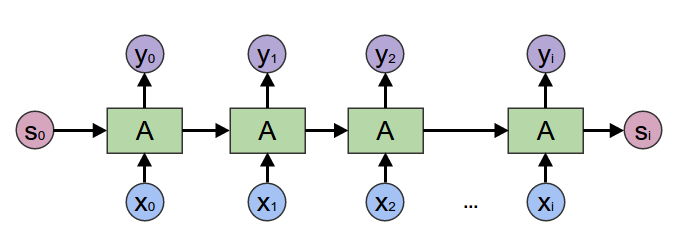
\includegraphics{/img/entries/functional-models/RNN-general.png}
\caption{Christopher Olah's RNN Unrolling Diagram}
\end{figure}

If we look at each one of those individual boxes, they all have two inputs
(normal input, and previous state) and two outputs (normal output, new state).

``Unrolling'' a stateful model means taking a model that takes in an \texttt{X}
and producing a \texttt{Y} and turning it into a model that takes an
\texttt{{[}X{]}} and produces a \texttt{{[}Y{]}}, by feeding it each of the
\texttt{X}s one after the other, propagating the state, and collecting all of
the \texttt{Y} responses.

The ``type'' of this sounds like:

\begin{Shaded}
\begin{Highlighting}[]
\OtherTok{unroll ::} \DataTypeTok{Model}\NormalTok{ p s a b }\OtherTok{->} \DataTypeTok{Model}\NormalTok{ p s [a] [b]}
\end{Highlighting}
\end{Shaded}

In writing this out as a type, we also note that the \texttt{p} parameter is the
same, and the \texttt{s} state type is the same. If you're familiar with
category theory, this looks a little bit like a sort of ``fmap'' under a
\texttt{Model\ p\ s} category -- it takes a \texttt{a\ -\textgreater{}\ b},
essentially, and turns it into an \texttt{{[}a{]}\ -\textgreater{}\ {[}b{]}}.

Olah's post suggests that this is a \texttt{mapAccum}, in functional programming
parlance. And, surely enough, we can actually write this as a
\texttt{mapAccumL}:

\begin{Shaded}
\begin{Highlighting}[]
\CommentTok{-- source: https://github.com/mstksg/inCode/tree/master/code-samples/functional-models/model.hs#L227-L235}

\NormalTok{unroll}
\OtherTok{    ::}\NormalTok{ (}\DataTypeTok{Traversable}\NormalTok{ t, }\DataTypeTok{Backprop}\NormalTok{ a, }\DataTypeTok{Backprop}\NormalTok{ b, }\DataTypeTok{Backprop}\NormalTok{ (t b))}
    \OtherTok{=>} \DataTypeTok{ModelS}\NormalTok{ p s a b}
    \OtherTok{->} \DataTypeTok{ModelS}\NormalTok{ p s (t a) (t b)}
\NormalTok{unroll f p xs s0 }\FunctionTok{=}\NormalTok{ swap }\FunctionTok{$}\NormalTok{ mapAccumL f' s0 xs}
  \KeywordTok{where}
    \CommentTok{-- we have to re-arrange the order of arguments and tuple a bit to}
    \CommentTok{-- match what `mapAccumL` expects}
\NormalTok{    f' s x }\FunctionTok{=}\NormalTok{ swap (f p x s)}
\end{Highlighting}
\end{Shaded}

This is \emph{exactly} the just the normal functional programming
\texttt{mapAccumL} of a stateful function over a container. And,
\texttt{mapAccumL} is general enough to be definable for all
\texttt{Traversable} containers (not just lists)! (We use \texttt{mapAccumL}
``lifted'' for \texttt{BVar}s from the
\emph{\href{http://hackage.haskell.org/package/backprop/docs/Prelude-Backprop.html}{Prelude.Backprop}}
module)

And, as normal functions, we can also get a version that gets only the ``final''
result:

\begin{Shaded}
\begin{Highlighting}[]
\CommentTok{-- source: https://github.com/mstksg/inCode/tree/master/code-samples/functional-models/model.hs#L237-L242}

\NormalTok{unrollLast}
\OtherTok{    ::}\NormalTok{ (}\DataTypeTok{Backprop}\NormalTok{ a, }\DataTypeTok{Backprop}\NormalTok{ b)}
    \OtherTok{=>} \DataTypeTok{ModelS}\NormalTok{ p s a b}
    \OtherTok{->} \DataTypeTok{ModelS}\NormalTok{ p s [a] b}
\NormalTok{unrollLast f }\FunctionTok{=}\NormalTok{ mapS (last }\FunctionTok{.}\NormalTok{ sequenceVar) (unroll f)}
\CommentTok{-- TODO: switch to (last . toList)}
\end{Highlighting}
\end{Shaded}

To see how this applies to our \texttt{threeLayer}:

\begin{Shaded}
\begin{Highlighting}[]
\OtherTok{threeLayers            ::} \DataTypeTok{ModelS}\NormalTok{ _ _ (}\DataTypeTok{R} \DecValTok{40}\NormalTok{) (}\DataTypeTok{R} \DecValTok{5}\NormalTok{)}
\NormalTok{unroll}\OtherTok{ threeLayers     ::} \DataTypeTok{ModelS}\NormalTok{ _ _ [}\DataTypeTok{R} \DecValTok{40}\NormalTok{] [}\DataTypeTok{R} \DecValTok{5}\NormalTok{]}
\NormalTok{unrollLast}\OtherTok{ threeLayers ::} \DataTypeTok{ModelS}\NormalTok{ _ _ [}\DataTypeTok{R} \DecValTok{40}\NormalTok{] (}\DataTypeTok{R} \DecValTok{5}\NormalTok{)}
\end{Highlighting}
\end{Shaded}

\hypertarget{state-be-gone}{%
\section{State-be-gone}\label{state-be-gone}}

Did you enjoy the detour through stateful time series models?

Good! Because the whole point of it was to talk about how we can get rid of
state and bring us back to our original models!

You knew this had to come, because all of our methods for ``training'' these
models and learn these parameters involves non-stateful models. Let's see now
how we can turn our functional stateful models into functional non-stateful
models!

One way is to \emph{fix the initial state and throw away the resulting one}.
This is very common in machine learning contexts, where many people simply fix
the initial state to be a zero vector.

\begin{Shaded}
\begin{Highlighting}[]
\CommentTok{-- source: https://github.com/mstksg/inCode/tree/master/code-samples/functional-models/model.hs#L244-L254}

\NormalTok{fixState}
\OtherTok{    ::}\NormalTok{ s}
    \OtherTok{->} \DataTypeTok{ModelS}\NormalTok{ p s a b}
    \OtherTok{->} \DataTypeTok{Model}\NormalTok{  p   a b}
\NormalTok{fixState s0 f p x }\FunctionTok{=}\NormalTok{ fst }\FunctionTok{$}\NormalTok{ f p x (constVar s0)}

\NormalTok{zeroState}
\OtherTok{    ::} \DataTypeTok{Num}\NormalTok{ s}
    \OtherTok{=>} \DataTypeTok{ModelS}\NormalTok{ p s a b}
    \OtherTok{->} \DataTypeTok{Model}\NormalTok{  p   a b}
\NormalTok{zeroState }\FunctionTok{=}\NormalTok{ fixState }\DecValTok{0}
\end{Highlighting}
\end{Shaded}

We use \texttt{constVar\ ::\ a\ -\textgreater{}\ BVar\ s\ a} again to introduce
a \texttt{BVar} of our initial state, but to indicate that we don't expect to
track its gradient. \texttt{zeroState} is a nice utility combinator for a common
design pattern.

Another way is to \emph{treat the initial state as a trainable parameter} (and
also throw away the final state). This is not done as often, but is still common
enough to be mentioned often. And, it's just as straightforward!

\begin{Shaded}
\begin{Highlighting}[]
\CommentTok{-- source: https://github.com/mstksg/inCode/tree/master/code-samples/functional-models/model.hs#L256-L263}

\NormalTok{trainState}
\OtherTok{    ::}\NormalTok{ (}\DataTypeTok{Backprop}\NormalTok{ p, }\DataTypeTok{Backprop}\NormalTok{ s)}
    \OtherTok{=>} \DataTypeTok{ModelS}\NormalTok{  p    s  a b}
    \OtherTok{->} \DataTypeTok{Model}\NormalTok{  (p }\FunctionTok{:&}\NormalTok{ s) a b}
\NormalTok{trainState f ps x }\FunctionTok{=}\NormalTok{ fst }\FunctionTok{$}\NormalTok{ f p x s}
  \KeywordTok{where}
\NormalTok{    p }\FunctionTok{=}\NormalTok{ ps }\FunctionTok{^^.}\NormalTok{ t1}
\NormalTok{    s }\FunctionTok{=}\NormalTok{ ps }\FunctionTok{^^.}\NormalTok{ t2}
\end{Highlighting}
\end{Shaded}

Essentially we take a model with trainable parameter \texttt{p} and state
\texttt{s}, and turn into a model with trainable parameter \texttt{p\ :\&\ s},
where the \texttt{s} is the initial state.

We can now \emph{train} our recurrent/stateful models, by \textbf{unrolling and
de-stating}:

\begin{Shaded}
\begin{Highlighting}[]
\OtherTok{threeLayers                        ::} \DataTypeTok{ModelS}\NormalTok{ _ _ (}\DataTypeTok{R} \DecValTok{40}\NormalTok{) (}\DataTypeTok{R} \DecValTok{5}\NormalTok{)}
\NormalTok{unrollLast}\OtherTok{ threeLayers             ::} \DataTypeTok{ModelS}\NormalTok{ _ _ [}\DataTypeTok{R} \DecValTok{40}\NormalTok{] (}\DataTypeTok{R} \DecValTok{5}\NormalTok{)}
\NormalTok{zeroState (unrollLast threeLayers)}\OtherTok{ ::} \DataTypeTok{Model}\NormalTok{  _   [}\DataTypeTok{R} \DecValTok{40}\NormalTok{] (}\DataTypeTok{R} \DecValTok{5}\NormalTok{)}
\end{Highlighting}
\end{Shaded}

\texttt{zeroState\ (unrollLast\ threeLayers)} is now a normal stateless (and
trainable) model. It takes a list of inputs \texttt{R\ 40}s and produces the
``final output'' \texttt{R\ 5}. We can now train this by feeding it with
\texttt{({[}R\ 40{]},\ R\ 5)} pairs: give a history and an expected next output.

Let's see this play out with our AR(2) model:

\begin{Shaded}
\begin{Highlighting}[]
\OtherTok{ar2                        ::} \DataTypeTok{ModelS}\NormalTok{ _ _ }\DataTypeTok{Double} \DataTypeTok{Double}
\NormalTok{unrollLast}\OtherTok{ ar2             ::} \DataTypeTok{ModelS}\NormalTok{ _ _ [}\DataTypeTok{Double}\NormalTok{] }\DataTypeTok{Double}
\NormalTok{zeroState (unrollLast ar2)}\OtherTok{ ::} \DataTypeTok{Model}\NormalTok{  _   [}\DataTypeTok{Double}\NormalTok{] }\DataTypeTok{Double}
\end{Highlighting}
\end{Shaded}

\texttt{zeroState\ (unrollLast\ ar2)} is now a trainable stateless model. Let's
use it to learn a sine wave:

\begin{Shaded}
\begin{Highlighting}[]
\CommentTok{-- sine signal with period 25}
\NormalTok{ghci}\FunctionTok{>}\NormalTok{ series }\FunctionTok{=}\NormalTok{ [ sin (}\DecValTok{2} \FunctionTok{*}\NormalTok{ pi }\FunctionTok{*}\NormalTok{ t }\FunctionTok{/} \DecValTok{25}\NormalTok{) }\FunctionTok{|}\NormalTok{ t }\OtherTok{<-}\NormalTok{ [}\DecValTok{0}\FunctionTok{..}\NormalTok{]              ]}
\CommentTok{-- chunks of runs and "next results"}
\NormalTok{ghci}\FunctionTok{>}\NormalTok{ samps  }\FunctionTok{=}\NormalTok{ [ (init c, last c)      }\FunctionTok{|}\NormalTok{ c }\OtherTok{<-}\NormalTok{ chunksOf }\DecValTok{19}\NormalTok{ series ]}
\NormalTok{ghci}\FunctionTok{>}\NormalTok{ trained }\OtherTok{<-}\NormalTok{ trainModelIO (zeroState (unrollLast ar2)) }\FunctionTok{$}\NormalTok{ take }\DecValTok{10000}\NormalTok{ samps}
\end{Highlighting}
\end{Shaded}

Trained! \texttt{trained} is the parameterization of \texttt{ar2} that will
simulate a sine wave of period 25.

Let's define some helper functions to test our model. First, a function
\texttt{prime} that takes a stateful model and gives a ``warmed-up'' state by
running it over a list of inputs. This will give the model a sense of ``where to
start''.

\begin{Shaded}
\begin{Highlighting}[]
\CommentTok{-- source: https://github.com/mstksg/inCode/tree/master/code-samples/functional-models/model.hs#L265-L272}

\NormalTok{prime}
\OtherTok{    ::} \DataTypeTok{Foldable}\NormalTok{ t}
    \OtherTok{=>} \DataTypeTok{ModelS}\NormalTok{ p s a b     }\CommentTok{-- ^ model}
    \OtherTok{->}\NormalTok{ p                  }\CommentTok{-- ^ parameterization}
    \OtherTok{->}\NormalTok{ s                  }\CommentTok{-- ^ initial state}
    \OtherTok{->}\NormalTok{ t a                }\CommentTok{-- ^ priming input}
    \OtherTok{->}\NormalTok{ s                  }\CommentTok{-- ^ primed state}
\NormalTok{prime f p }\FunctionTok{=}\NormalTok{ foldl' }\FunctionTok{$}\NormalTok{ evalBP2 (\textbackslash{}s x }\OtherTok{->}\NormalTok{ snd }\FunctionTok{$}\NormalTok{ f (constVar p) x s)}
\end{Highlighting}
\end{Shaded}

Then a function \texttt{feedback} that iterates a stateful model over and over
again by feeding its previous output as its next input:

\begin{Shaded}
\begin{Highlighting}[]
\CommentTok{-- source: https://github.com/mstksg/inCode/tree/master/code-samples/functional-models/model.hs#L278-L287}

\NormalTok{    return }\FunctionTok{.}\NormalTok{ take }\DecValTok{50} \FunctionTok{$}\NormalTok{ feedback model0 trained primed (series }\FunctionTok{!!} \DecValTok{20}\NormalTok{)}
  \KeywordTok{where}
    \CommentTok{-- sine wave with period 25}
\OtherTok{    series ::}\NormalTok{ [}\DataTypeTok{Double}\NormalTok{]}
\NormalTok{    series }\FunctionTok{=}\NormalTok{ [ sin (}\DecValTok{2} \FunctionTok{*}\NormalTok{ pi }\FunctionTok{*}\NormalTok{ t }\FunctionTok{/} \DecValTok{25}\NormalTok{) }\FunctionTok{|}\NormalTok{ t }\OtherTok{<-}\NormalTok{ [}\DecValTok{0}\FunctionTok{..}\NormalTok{]              ]}
\NormalTok{    samps  }\FunctionTok{=}\NormalTok{ [ (init c, last c)      }\FunctionTok{|}\NormalTok{ c }\OtherTok{<-}\NormalTok{ chunksOf }\DecValTok{19}\NormalTok{ series ]}
\OtherTok{    model0 ::} \DataTypeTok{ModelS}\NormalTok{ _ _ }\DataTypeTok{Double} \DataTypeTok{Double}
\NormalTok{    model0 }\FunctionTok{=}\NormalTok{ ar2}
\OtherTok{    model  ::} \DataTypeTok{Model}\NormalTok{  _   [}\DataTypeTok{Double}\NormalTok{] }\DataTypeTok{Double}
\NormalTok{    model  }\FunctionTok{=}\NormalTok{ zeroState }\FunctionTok{$}\NormalTok{ unrollLast model0}
\end{Highlighting}
\end{Shaded}

Now let's prime our trained model over the first 19 items in our sine wave and
start it running in feedback mode on the 20st item!

\begin{Shaded}
\begin{Highlighting}[]
\NormalTok{ghci}\FunctionTok{>} \KeywordTok{let}\NormalTok{ primed }\FunctionTok{=}\NormalTok{ prime    ar2 trained }\DecValTok{0}\NormalTok{      (take }\DecValTok{19}\NormalTok{ series)}
\NormalTok{ghci}\FunctionTok{>} \KeywordTok{let}\NormalTok{ output }\FunctionTok{=}\NormalTok{ feedback ar2 trained primed (series }\FunctionTok{!!} \DecValTok{20}\NormalTok{)}
\NormalTok{ghci}\FunctionTok{>}\NormalTok{ mapM_ print }\FunctionTok{$}\NormalTok{ take }\DecValTok{30}\NormalTok{ output}
\FunctionTok{-}\FloatTok{0.9510565162951536}
\FunctionTok{-}\FloatTok{0.8600674032037106}
\FunctionTok{-}\FloatTok{0.7150370920644853}
\FunctionTok{-}\FloatTok{0.5250783707105848}
\FunctionTok{-}\FloatTok{0.302127044224051}
\FunctionTok{-}\FloatTok{6.019196440573038e-2}
\FloatTok{0.18552519790433009}
\FloatTok{0.41958512971360296}
\FloatTok{0.627280984694227}
\FloatTok{0.795562468425788}
\FloatTok{0.9138558363893832}
\FloatTok{0.9747282812232584}
\FloatTok{0.9743549633453022}
\FloatTok{0.9127593396907665}
\FloatTok{0.7938116898267549}
\FloatTok{0.6249859320531274}
\FloatTok{0.41689000962856815}
\FloatTok{0.18259935468235244}
\FunctionTok{-}\FloatTok{6.316468927441621e-2}
\FunctionTok{-}\FloatTok{0.3049598635029274}
\FunctionTok{-}\FloatTok{0.5275932879458836}
\FunctionTok{-}\FloatTok{0.7170760857570087}
\FunctionTok{-}\FloatTok{0.861502355880794}
\FunctionTok{-}\FloatTok{0.9517972646026605}
\FunctionTok{-}\FloatTok{0.9822872507261515}
\FunctionTok{-}\FloatTok{0.9510565162888059}
\FunctionTok{-}\FloatTok{0.8600674031939511}
\FunctionTok{-}\FloatTok{0.7150370920519272}
\FunctionTok{-}\FloatTok{0.5250783706960173}
\FunctionTok{-}\FloatTok{0.3021270442083892}
\end{Highlighting}
\end{Shaded}

Looks like a beautiful sine wave! It starts out at -0.95, gradually rolls back
towards 0, cross over and peaks out at positive 0.97, then swings back around
past zero and reaches a minimum at -0.97 before swinging back again. Pretty much
a perfect sine wave with period 25. AR(2) works pretty well!

For kicks, let's try it with a two-layer fully connected neural network with 20
hidden units, where the first layer is fully recurrent:

\begin{Shaded}
\begin{Highlighting}[]
\CommentTok{-- first layer is RNN, second layer is normal ANN, 20 hidden units}
\NormalTok{ghci}\FunctionTok{>} \KeywordTok{let}\OtherTok{ rnn ::} \DataTypeTok{ModelS}\NormalTok{ _ _ (}\DataTypeTok{R} \DecValTok{1}\NormalTok{) (}\DataTypeTok{R} \DecValTok{1}\NormalTok{)}
\NormalTok{          rnn }\FunctionTok{=}\NormalTok{ feedForward }\FunctionTok{@}\DecValTok{20} \FunctionTok{@}\DecValTok{1} \FunctionTok{<*~}\NormalTok{ mapS logistic (fcrnn }\FunctionTok{@}\DecValTok{1} \FunctionTok{@}\DecValTok{20}\NormalTok{)}
\NormalTok{ghci}\FunctionTok{>}\NormalTok{ trained }\OtherTok{<-}\NormalTok{ trainModelIO (trainZero (unrollLast rnn)) }\FunctionTok{$}\NormalTok{ take }\DecValTok{10000}\NormalTok{ samps}
\NormalTok{ghci}\FunctionTok{>} \KeywordTok{let}\NormalTok{ primed }\FunctionTok{=}\NormalTok{ prime    rnn trained }\DecValTok{0}\NormalTok{      (take }\DecValTok{19}\NormalTok{ series)}
\NormalTok{ghci}\FunctionTok{>} \KeywordTok{let}\NormalTok{ output }\FunctionTok{=}\NormalTok{ feedback rnn trained primed (series }\FunctionTok{!!} \DecValTok{20}\NormalTok{)}
\NormalTok{ghci}\FunctionTok{>}\NormalTok{ mapM_ print }\FunctionTok{$}\NormalTok{ take }\DecValTok{30}\NormalTok{ output}
\NormalTok{(}\FunctionTok{-}\FloatTok{0.9510565162951536}\OtherTok{ ::} \DataTypeTok{R} \DecValTok{1}\NormalTok{)}
\NormalTok{(}\FunctionTok{-}\FloatTok{0.8513651168000752}\OtherTok{ ::} \DataTypeTok{R} \DecValTok{1}\NormalTok{)}
\NormalTok{(}\FunctionTok{-}\FloatTok{0.7166599836716709}\OtherTok{ ::} \DataTypeTok{R} \DecValTok{1}\NormalTok{)}
\NormalTok{(}\FunctionTok{-}\FloatTok{0.5482473595389897}\OtherTok{ ::} \DataTypeTok{R} \DecValTok{1}\NormalTok{)}
\NormalTok{(}\FunctionTok{-}\FloatTok{0.34915724320186287}\OtherTok{ ::} \DataTypeTok{R} \DecValTok{1}\NormalTok{)}
\NormalTok{(}\FunctionTok{-}\FloatTok{0.12410494333456273}\OtherTok{ ::} \DataTypeTok{R} \DecValTok{1}\NormalTok{)}
\NormalTok{(}\FloatTok{0.11796522261125514}\OtherTok{ ::} \DataTypeTok{R} \DecValTok{1}\NormalTok{)}
\NormalTok{(}\FloatTok{0.3617267605713303}\OtherTok{ ::} \DataTypeTok{R} \DecValTok{1}\NormalTok{)}
\NormalTok{(}\FloatTok{0.5859020418343457}\OtherTok{ ::} \DataTypeTok{R} \DecValTok{1}\NormalTok{)}
\NormalTok{(}\FloatTok{0.768017196984538}\OtherTok{ ::} \DataTypeTok{R} \DecValTok{1}\NormalTok{)}
\NormalTok{(}\FloatTok{0.8918483864333885}\OtherTok{ ::} \DataTypeTok{R} \DecValTok{1}\NormalTok{)}
\NormalTok{(}\FloatTok{0.9520895380310987}\OtherTok{ ::} \DataTypeTok{R} \DecValTok{1}\NormalTok{)}
\NormalTok{(}\FloatTok{0.9527522551095625}\OtherTok{ ::} \DataTypeTok{R} \DecValTok{1}\NormalTok{)}
\NormalTok{(}\FloatTok{0.9018819269836273}\OtherTok{ ::} \DataTypeTok{R} \DecValTok{1}\NormalTok{)}
\NormalTok{(}\FloatTok{0.8071298312549686}\OtherTok{ ::} \DataTypeTok{R} \DecValTok{1}\NormalTok{)}
\NormalTok{(}\FloatTok{0.6739841516649296}\OtherTok{ ::} \DataTypeTok{R} \DecValTok{1}\NormalTok{)}
\NormalTok{(}\FloatTok{0.5060989906080221}\OtherTok{ ::} \DataTypeTok{R} \DecValTok{1}\NormalTok{)}
\NormalTok{(}\FloatTok{0.3068094725343112}\OtherTok{ ::} \DataTypeTok{R} \DecValTok{1}\NormalTok{)}
\NormalTok{(}\FloatTok{8.132150399626142e-2}\OtherTok{ ::} \DataTypeTok{R} \DecValTok{1}\NormalTok{)}
\NormalTok{(}\FunctionTok{-}\FloatTok{0.16084964907608051}\OtherTok{ ::} \DataTypeTok{R} \DecValTok{1}\NormalTok{)}
\NormalTok{(}\FunctionTok{-}\FloatTok{0.404157125663194}\OtherTok{ ::} \DataTypeTok{R} \DecValTok{1}\NormalTok{)}
\NormalTok{(}\FunctionTok{-}\FloatTok{0.6277521119177744}\OtherTok{ ::} \DataTypeTok{R} \DecValTok{1}\NormalTok{)}
\NormalTok{(}\FunctionTok{-}\FloatTok{0.8099883239222189}\OtherTok{ ::} \DataTypeTok{R} \DecValTok{1}\NormalTok{)}
\NormalTok{(}\FunctionTok{-}\FloatTok{0.9351261952804909}\OtherTok{ ::} \DataTypeTok{R} \DecValTok{1}\NormalTok{)}
\NormalTok{(}\FunctionTok{-}\FloatTok{0.9975997729210249}\OtherTok{ ::} \DataTypeTok{R} \DecValTok{1}\NormalTok{)}
\NormalTok{(}\FunctionTok{-}\FloatTok{1.000820693251437}\OtherTok{ ::} \DataTypeTok{R} \DecValTok{1}\NormalTok{)}
\NormalTok{(}\FunctionTok{-}\FloatTok{0.9525015209823966}\OtherTok{ ::} \DataTypeTok{R} \DecValTok{1}\NormalTok{)}
\NormalTok{(}\FunctionTok{-}\FloatTok{0.8603987544425211}\OtherTok{ ::} \DataTypeTok{R} \DecValTok{1}\NormalTok{)}
\NormalTok{(}\FunctionTok{-}\FloatTok{0.7303128941490123}\OtherTok{ ::} \DataTypeTok{R} \DecValTok{1}\NormalTok{)}
\NormalTok{(}\FunctionTok{-}\FloatTok{0.5660763612885787}\OtherTok{ ::} \DataTypeTok{R} \DecValTok{1}\NormalTok{)}
\end{Highlighting}
\end{Shaded}

Also looks nice! Notice that on the second negative peak, the network just
perfectly hits -1.00, which is exactly where it's supposed to turn around.
Sounds like an ``unreasonably effective'' recurrent neural network!

\end{document}
